\documentclass{scrartcl}
\usepackage[utf8]{inputenc}
\usepackage[english]{babel} % Trennung nach der neuen deutschen Rechtschreibung
\usepackage[utf8]{inputenc}
\usepackage[T1]{fontenc}
\usepackage{lmodern}

\usepackage{amsmath} % Erweiterte Mathematik-Umgebung
\usepackage{amsfonts} % zusätzliche Mathematik-Schrifttypen (v.a. \mathbb für Mengen)
\usepackage{ulem}

\usepackage{graphics}%soll beim Graphiken einfügen hilfreich sein
\usepackage{graphicx}
\usepackage{wrapfig}%lässt Textumflossene Bildeinbindung zu
\usepackage{epstopdf}%soll eps in pdf umwandeln

\usepackage[a4paper, portrait, margin=2.5cm]{geometry}

\titlehead{\centering University of Luxemburg}
\subject{Travaux Pratiques}
\title{Mechanical Oscillator}
\subtitle{Sergey Ershov}
\date{TP Session 22/10/2021}
\author{Louis-Hendrik Barboutie \\ Frederik Ehl \\ Florence Schmerber}

\begin{document}

\maketitle

\clearpage

\tableofcontents
\listoffigures
	
\clearpage


\section{Introduction}

During this experiment, we want to understand the characteristics of a mechanical oscillator, in particular the oscillation amplitude for different types of oscillators, like one that can oscillate freely, which is imposed by a damping factor and one who is powered by an electrical motor. We will also discuss the resonance phenomenon that we will encounter in this experiment as well as the principle of a transient/steady state and finally the beat and bandwidth of the oscillation.

\section{Experimental setup}

The mechanical oscillator is composed of a metal disk, that is attached to the rotation axis, a spring and a Eddy current brake. This freely oscillating movement is characterised by its angular velocity $\Omega$ and the dampening constant $\gamma$.

\medskip
\begin{figure} [h]
    \centering
    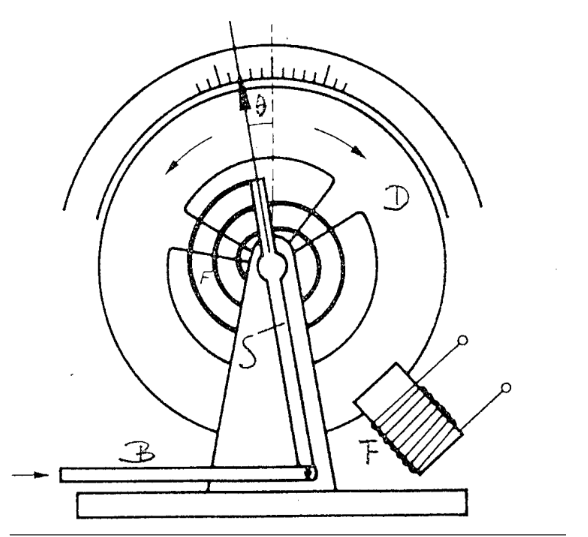
\includegraphics[width=6cm]{Mechanical_Oscillator.PNG}
    \caption{Mechanical Oscillator}
    \label{fig:}
\end{figure}

\section{Results}

\subsection{Pre-experimental discussion}

A free oscillator system will be exited by an exterior motor, which gradually imposes its own oscillation onto the system. We can then notice two states: First the system is in a transient state, where the amplitude of the oscillation is not constant and varies a lot. The two different angular velocities ($\omega \neq \Omega$) of both the imposed and the initial oscillations superpose. Then the system enters a steady state where the amplitude of the oscillation stays the same and the oscillations overlap.

We first want to discuss the equation given in the handout of this experiment:

\begin{equation}
    \Theta(t)=[A-A_0e^{-\gamma t}+2A_0e^{-\gamma t}cos(\frac{\omega-\omega_0}{2})t]sin(\omega t)
\end{equation}
%This equation is the general solution for the homogeneous oscillation equation.

The first term $A=A(\omega)$ is the amplitude of the exterior oscillation imposed on the disc. It depends on the imposed pulsation and does not decrease exponentially. This term shows the amplitude of the steady state.
The second term, $A_0e^{-\gamma t}$ takes into account the inertia of the pendulum. It depends on the initial amplitude $A_0$ and of the damping constant $\gamma$. This term represents an exponential decay, , which is the time during which the new forced angular frequency is being opposed the the inertia of the oscillator.
And the last term $2A_0e^{-\gamma t}cos(\frac{\omega-\omega_0}{2})t$ describes the beat of the transient state.

\begin{itemize}
    \item We can define the beat frequency $f_s$ as:
    \begin{equation}
        f_s=|f_1-f_2|\nonumber
    \end{equation}
    which gives us transforming f into $\omega$:
    \begin{equation}
        \omega_s=|\Omega-\omega|\nonumber
    \end{equation}
    \item If we want to see strong changes in the amplitude, we need to give the oscillation time to resonate in order for them to be observable.  We choose a weak damping for this, so that the damping effect does not slow the oscillator down until stopping.
    \item If we want to see an observable change in amplitudes called ”bulges” during the transient state, we need to produce multiple  cycles  of  alternating  destructive  and  constructive  superposition  to  take  place. That’s why we choose a larger $\omega$, and preferably a multiple of $\omega_0$
\end{itemize}

\subsection{Determining the angular velocity of the exterior oscillation} 

For this part of the experiment, we consider there to be no damping effect ($\gamma = 0$). We will be studying the exterior oscillation imposed by a motor for different voltages (between 8-10V), that means we don't consider the "main" oscillation. For that, we measure the time it takes for the arm of the motor to make 10 turns, which we will call $t_{10}$, for different voltages. Due to a malfunction of our equipment, our voltage could not be stabilized . So to get $T$ we simply use the relation: $T=\frac{t_{10}}{10}$. That way we get a more precise value for the period.
Knowing $T$ for each corresponding voltages, we can calculate the angular velocity $\omega$ for each corresponding $T$ with:

\begin{equation}
    \omega(U)=\frac{2\pi}{T(U)}
\end{equation}

\begin{figure}[h]
    \centering
    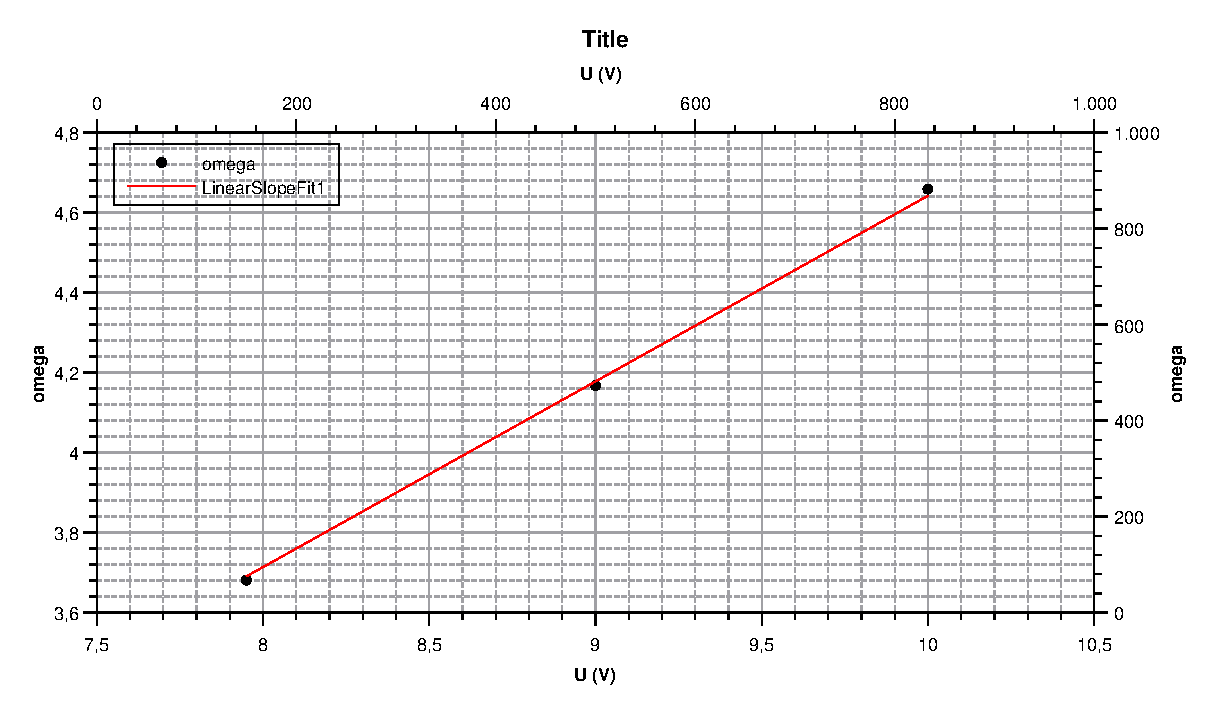
\includegraphics[width = 12cm]{SLopeOsci.eps}
    \caption{Omega as function of Voltage}
    \label{fig:my_label}
\end{figure}

The slope of the our linear fit is: 0,4641945
%We can see that T decreases constantly with the increase of voltage 

\subsection{Determining the period of a mechanical oscillator with and without damping}

Now we want to study the oscillator but this time without the motor. We will be measuring the time for 10 oscillations for 3 different dampening factors. First without friction, which means $I_0=0A$ and then for two different currents applied the Eddy current brake: $I_1= 0,25A$ and $I_2= 0,35A$. Then we divide the time we measured by 10 to get $T$, one full period. We first take the measurement manually with a stopwatch and a second time with a sensor attached to the oscillator. We will be plotting the results from the sensor on Qtiplot and measure the time of 10 peeks, then divide that by 10 to get one period. Then we cam easily calculate the angular velocity by using $\Omega=\frac{2\pi}{T}$. By doing it with two different methods we get a more precise result.

\medskip
\centering
\begin{tabular}{|c|c|c|c|}
    \hline
    $ $ & $ t_{I_0} $ & $ t_{I_1} $ & $ t_{I_2} $\\
    \hline
    $manually$ & $ 18,44 $ & $ 18,42$ & $18,6$  \\
    \hline
    $sensor$ & $ 18,3348 $ & $ 18,2724$ & $ 18,4304$  \\
    \hline
    $average$ & $ 18,3874 $ & $ 18,3462 $ & $18,5152$  \\
    \hline
\end{tabular}
\medskip

\centering
\begin{tabular}{|c|c|c|c|}
    \hline
    $ $ & $ T_{I_0} $ & $ T_{I_1} $ & $ T_{I_2} $\\
    \hline
    $average$ & $ 1,839 $ & $ 1,835 $ & $1,852$ \\
    \hline
    $\Omega$ & $ 3,42 $ & $ 3,41 $ & $ 3,39 $ \\
    \hline
\end{tabular}
\flushleft

%insert comments and observations

\subsection{Determining the dampening constants}

For this part of the experiment we want to determine the different dampening constants $\gamma_1$ and $\gamma_2$.
We look at our plotting of the oscillations we got previously (see appendix) and can determine the amplitude at the beginning of the oscillations and at the end, after 10 periods.
Using the logarithmic decrement we calculate $\gamma T$ with our values, where n=10:
\begin{equation}
    \gamma T = \frac{1}{n} ln(\frac{\Theta(t)}{\Theta(t+nT)})
\end{equation}

From this equation we compute $\gamma$:

\centering
\begin{tabular}{|c|c|c|c|}
    \hline
     & $I_0$ & $I_1$ & $I_2$ \\
     \hline
    $\gamma$ & $0,005$ & $0,06$ & $0,11$ \\
    \hline
\end{tabular}
\flushleft

Logarithmic decrement, is used to find the damping ratio of an underdamped system in the time domain.
For the following we make the assumption that we have small damping, meaning $\omega_0^2>>\gamma^2$, which we can verify since in our case they differ by a factor of $\approx500.000$ . For the ratio of $\gamma_2 / \gamma_1$ we obtain a value of $\approx 1,821$.

%bande passante : 7,521-7,296 V
%bande passant / 2 = gamma = 0,1125

\subsection{Determining the resonance frequency}

For this last part we want to determine the resonance frequency.
%we cam also calculate again the dampening constant + compare.
We know that $\Omega_{res}=\sqrt{\Omega_0^2-2\gamma^2}$ and with the approximation we did earlier we have $\Omega_{res}\approx\Omega_0$. This is a good starting point for our search for the resonance frequency. To impose $\Omega_0$ to the oscillator we need to find the corresponding voltage for the exterior oscillator. Therefore we use the relation between the Voltage and the angular frequency of the exterior oscillator $U_0=\frac{\Omega_0}{a}$, where a is the slope found in part one. We find a Voltage of 7,43V. When applying that specific voltage (with dampening I=0,25A) and starting the software of the sensor to plot the oscillation we can identify first the transient state and then the steady state. We wait one to two minutes so that we can measure the amplitude at the steady state. We then vary the Voltage in multiple steps of 0,2V around $U_0$ and note the obtained amplitude. We need to reconvert the different Voltages back into angular frequencies. With these results, we can plot a graph for the different amplitudes, where we can identify the resonance frequency from the maximum amplitude, as well as the bandwidth. The bandwidth is the range of $\Omega$ for which a value of at least $\frac{A_{res}}{\sqrt{2}}$ is attained. The bandwidth is also equal to $2\gamma$.
We use this relation to determine $\gamma_2$ again. We obtain $\Delta \omega \approx (w2-w1)=0,1 \ rad \cdot s^{-1}$ and deduce $\gamma = \frac{\Delta \omega}{2} \approx 0,5$ which is 17\% smaller than the value we determined in the last section.
\newline

\textit{Remark: Our oscillator wasn't working properly, that's why our results aren't accurate. Our supervisor gave us the correct values in order for us to continue}

\section{Conclusion}
In the first part of the experiment, we observed forced oscillations, driven by an exterior motor. We derived a linear relationship between the angular frequency and the voltage U that we applied to the motor and deduced a function for $\omega(U)$. In the second part of the experiment, we observed that the damping of the Eddy current brake does not impact the period T of the mechanical oscillator. The goal of the third part of the experiment was to determine the values of the damping constants for different applied currents to the current brake. With the logarithmic decrement we obtained the following values: $\gamma_0=0,005Hz$, $\gamma_1=0,06Hz$ and $\gamma_2=0,11Hz$ with a ratio $\frac{\gamma_2}{\gamma_1}\approx1,821$. In the last part of the experiment, we studied the phenomenon of resonance. By constructing a graph we were able to deduce the resonance frequency and the bandwidth of the function. This also served as a way to recalculate the damping factor $\gamma$ again, where we obtained a value of $\gamma_1\approx0,5Hz$ which deviated by $17\%$ from our first calculation. 


\section{Appendix}

\begin{figure}[h]
    \centering
    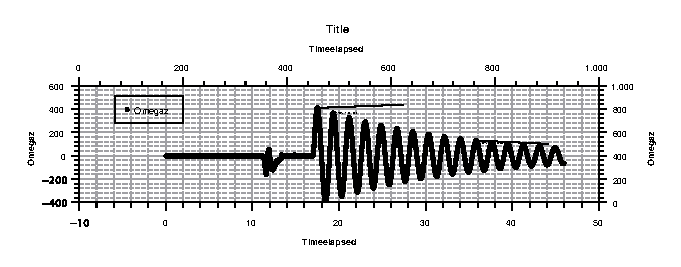
\includegraphics[width=16cm]{Graph1.eps}
    \caption{Damped Oscillator 0.25A}
    \label{fig:}
\end{figure}

\begin{figure}[h]
    \centering
    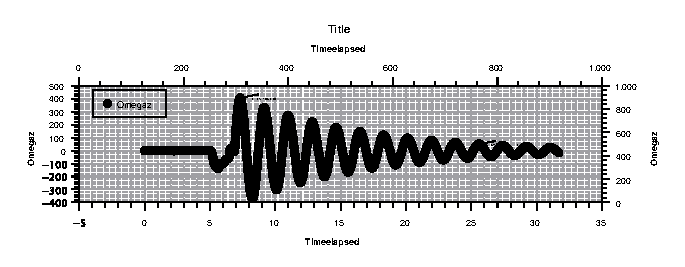
\includegraphics[width=16cm]{Graph2.eps}
    \caption{Damped Oscillator 0,35A}
    \label{fig:}
\end{figure}

\begin{figure}
    \centering
    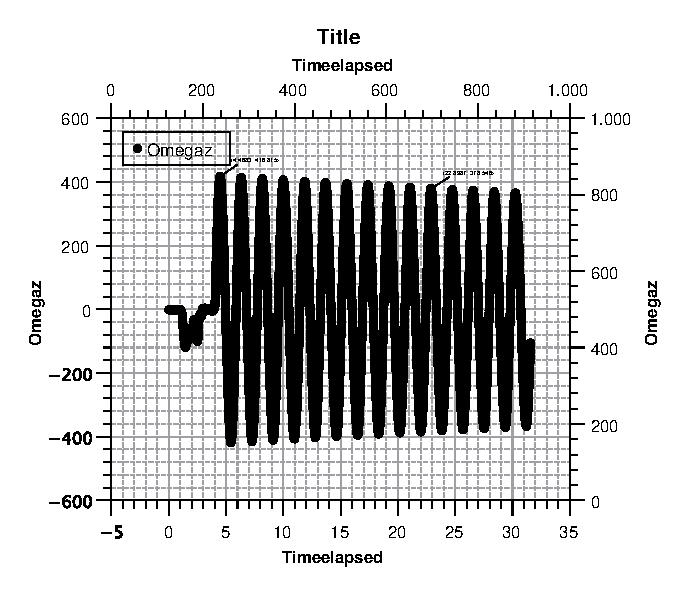
\includegraphics[width=12cm]{Graph3.eps}
    \caption{Free Oscillator}
    \label{fig:}
\end{figure}


\end{document}